\subsection{Abstract}

This project focuses on modifying a 3D printer to create chocolate sculptures.
Achieving this required changes to both the hardware and software.

\subsection{Showcase}

\begin{center}
    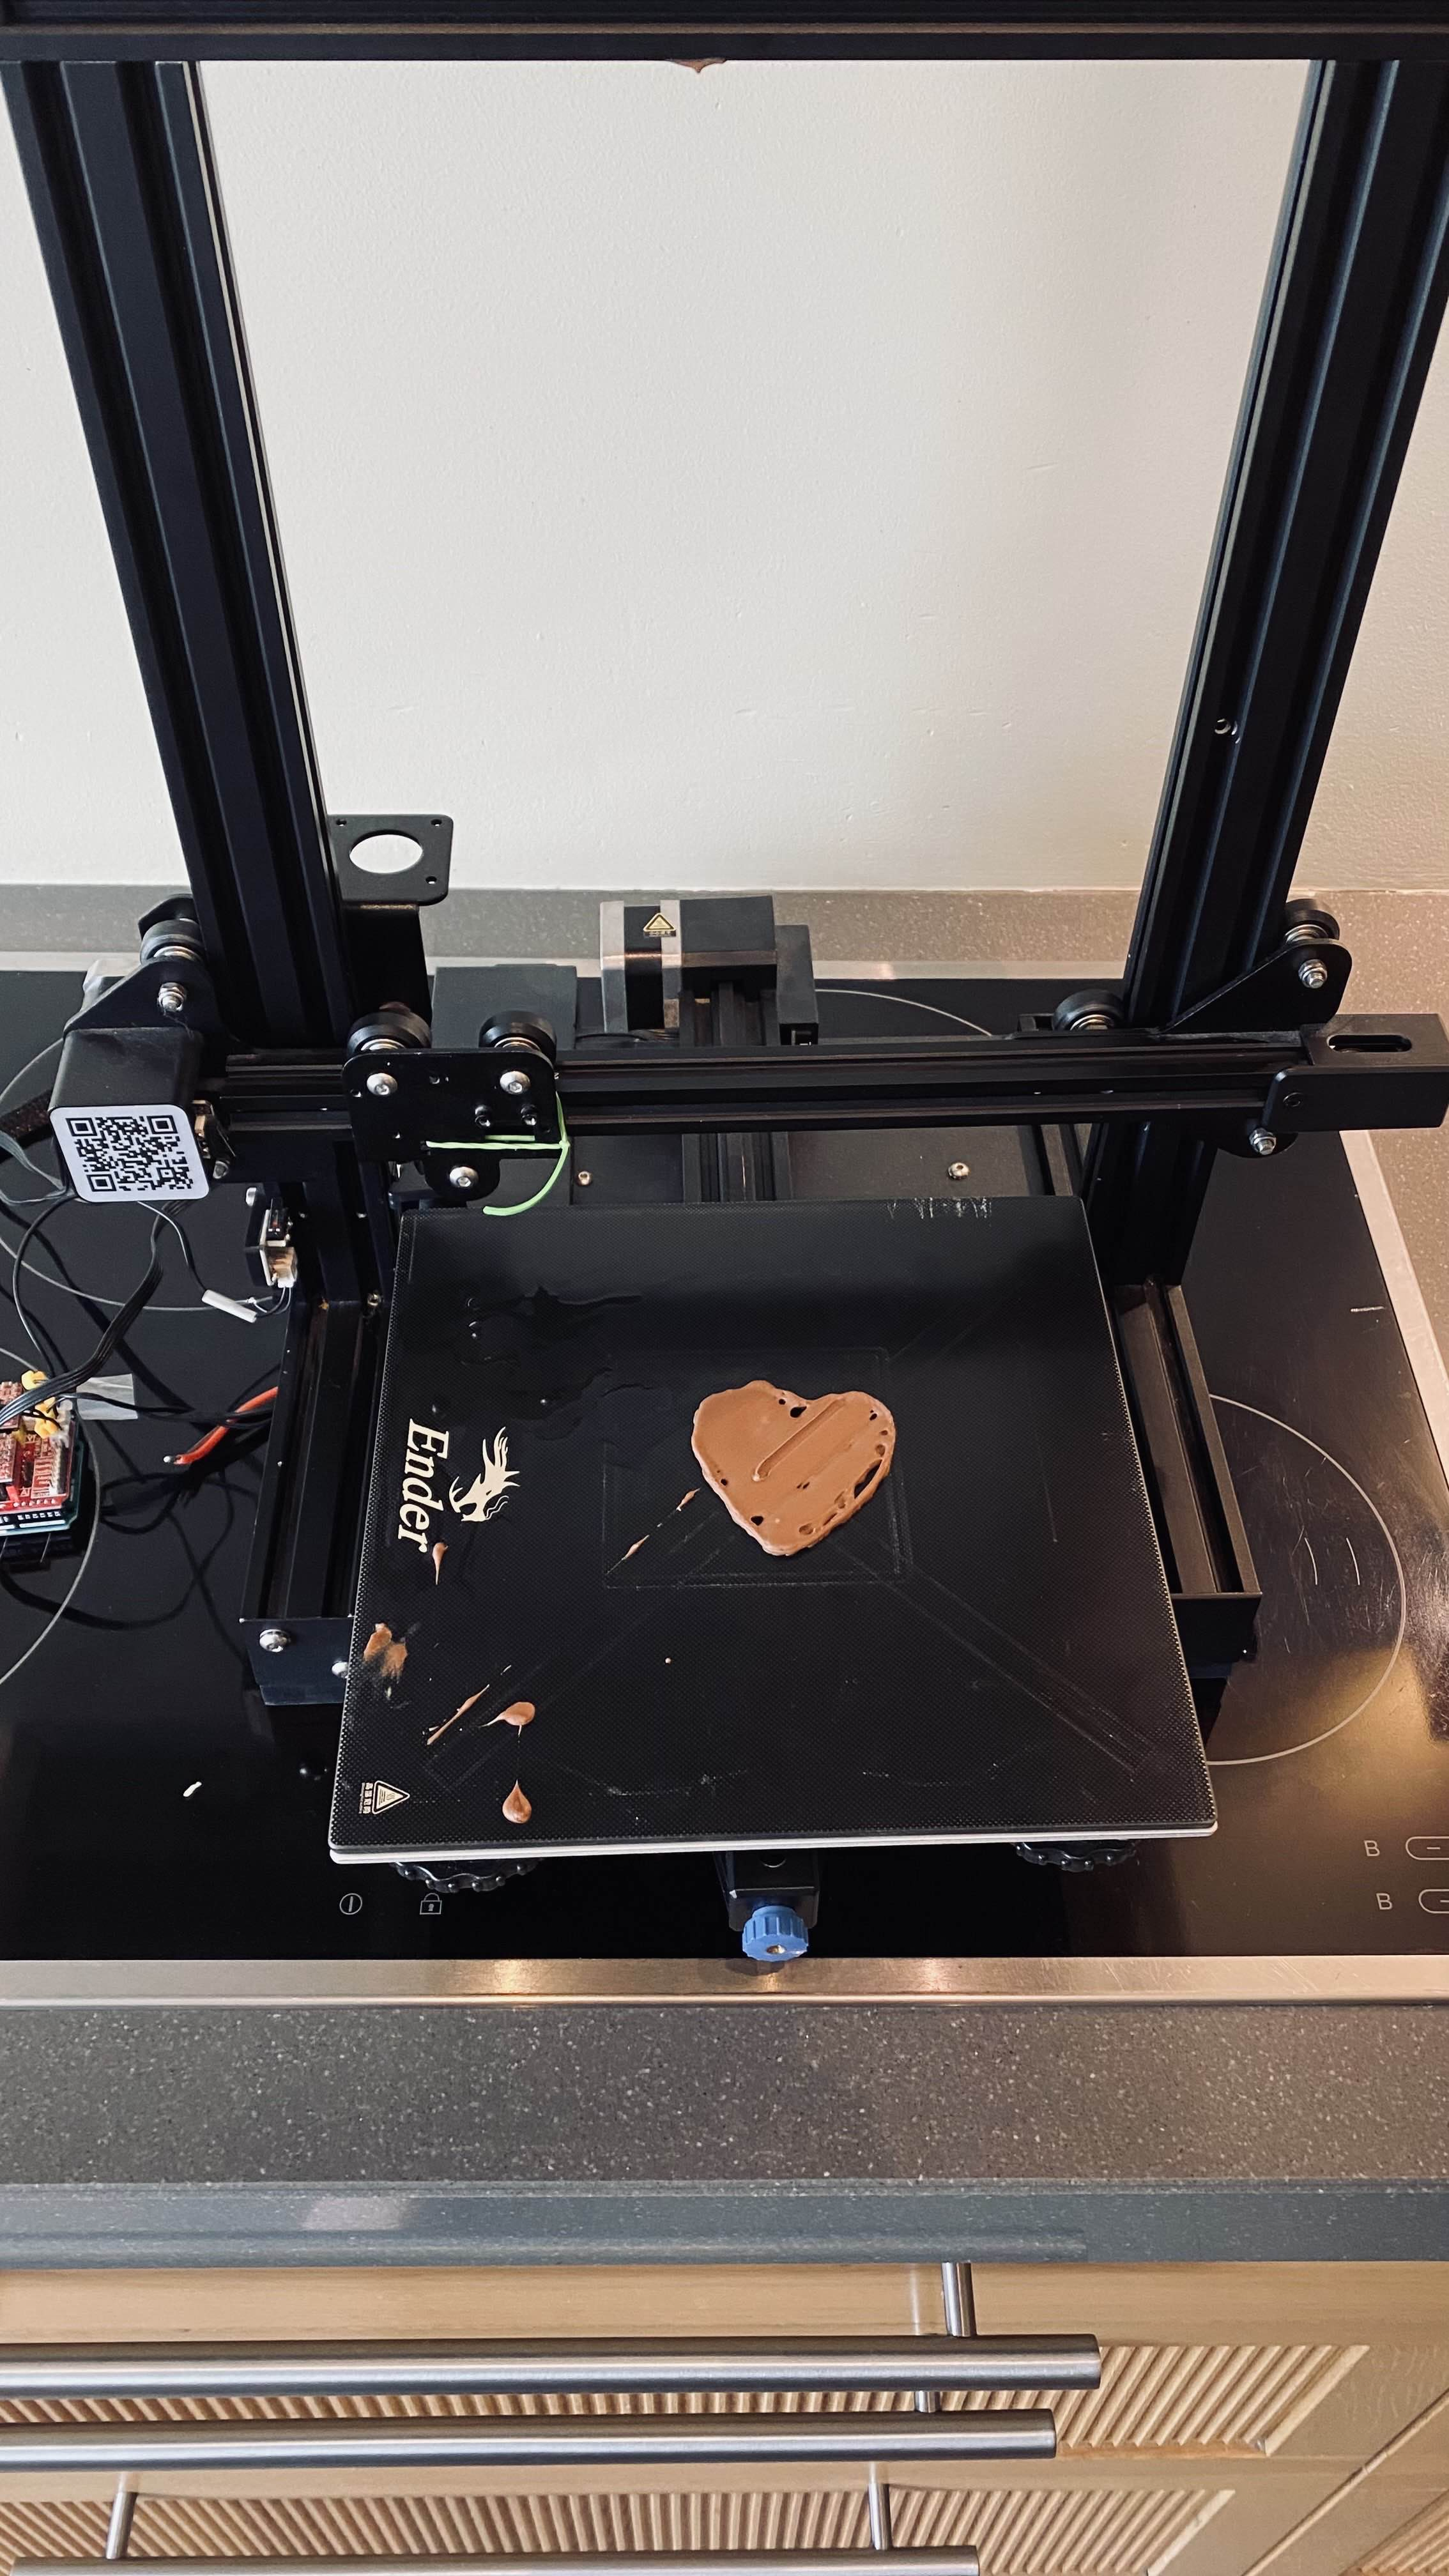
\includegraphics[width=0.2\textwidth]{introduction/hart.jpg}
\end{center}

\subsection{Project Overview}

\begin{center}
    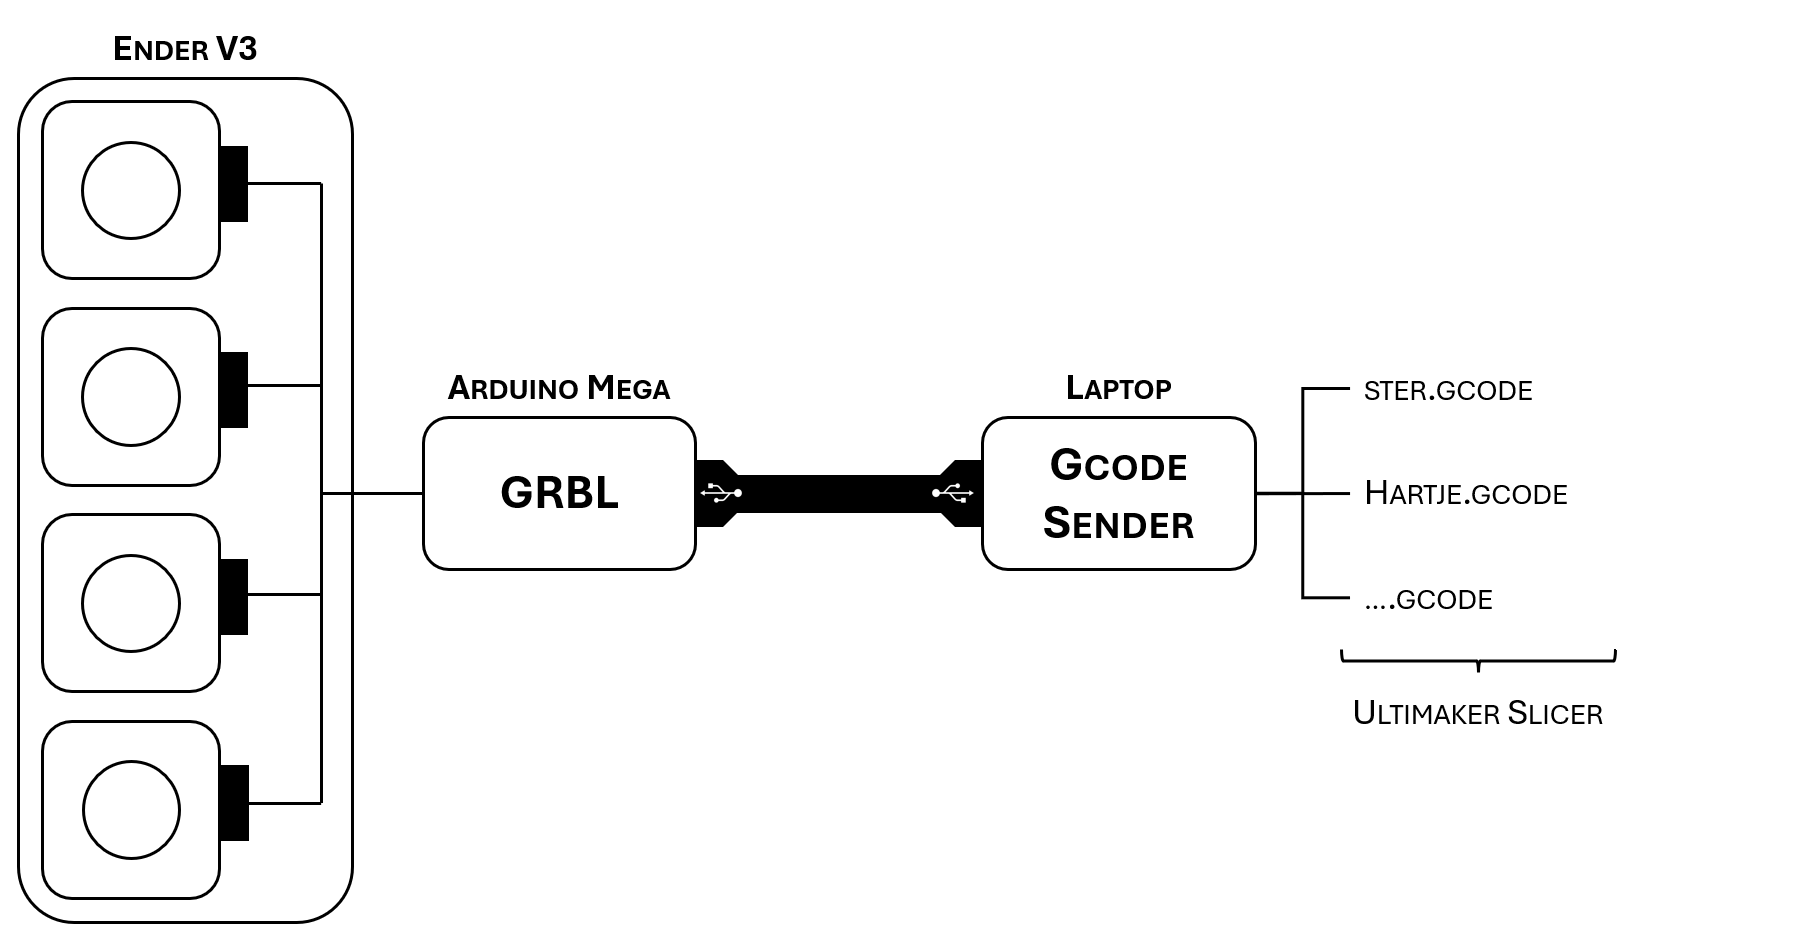
\includegraphics[width=0.7\textwidth]{introduction/overview.png}
\end{center}

Herwith I provide a high-level overview of this project.
When you want to print a 3d file, you shall first slice it in a 3d program
like Ultimaker Slicer. After that, you import the .gcode file into the gcode sender.
This is a python Graphical User Interface that communicates with the printer to
monitor its temperature etc. When you press play in the gcode sender, it starts sending
commands to the printer's controller. That is an arduino, running modified GRBL software.
The arduino gets commands like "move to this position at this speed, while extruding this much
chocolate". And finally the arduino will controll its stepper motors so that these commands
are executed.

\newpage % intended for later use

\subsection{Timeline}
To be completed.